\begin{figure}
\centering
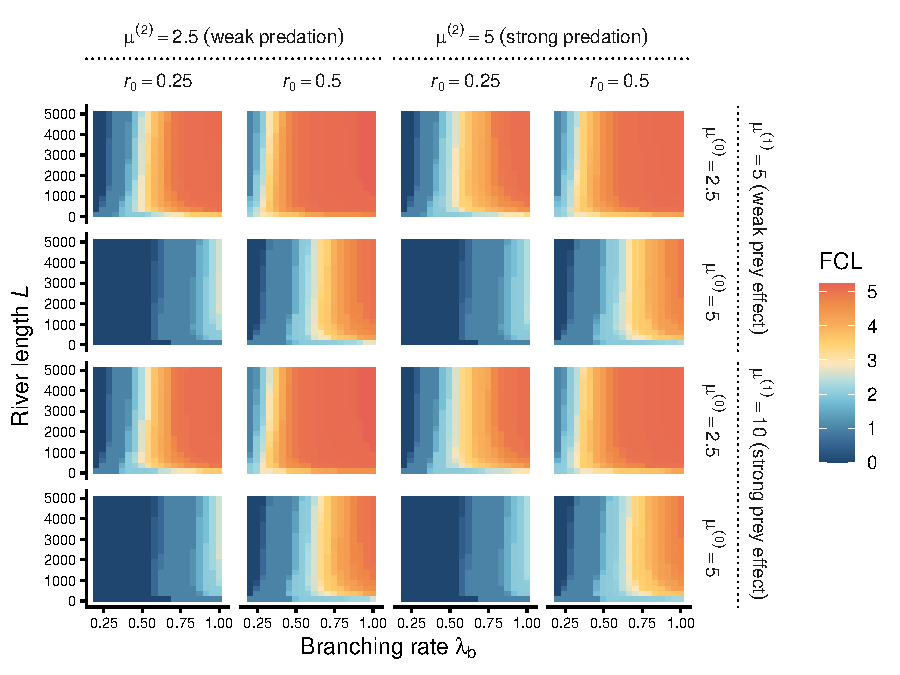
\includegraphics[width=1\linewidth]{tex/fig_theo_delta01_nu01_theta025.pdf}
\caption{Numerical predictions with dispersal decay rate $\delta_0 = 0.1$ (for producers), disturbance decay rate $\nu = 0.1$, and weak omnivory $\theta = 0.25$. Heatmaps of FCL are expressed as a function of ecosystem size (river length, $L$)
and complexity (branching rate, $\lambda_b$), with rows and columns displaying
different combinations of resource supply ($r_0$), disturbance regime
($\mu^{(0)}$), prey effect ($\mu^{(1)}$), and predation effect ($\mu^{(2)}$).
Each cell represents the average FCL of five food webs.
Other parameter values are: producer propagule $g_0 = 5$, habitat density $h = 1$, scaling exponent $\psi = 0.5$.}
\label{fig:fig-num1}
\end{figure}
\newpage

\begin{figure}
\centering
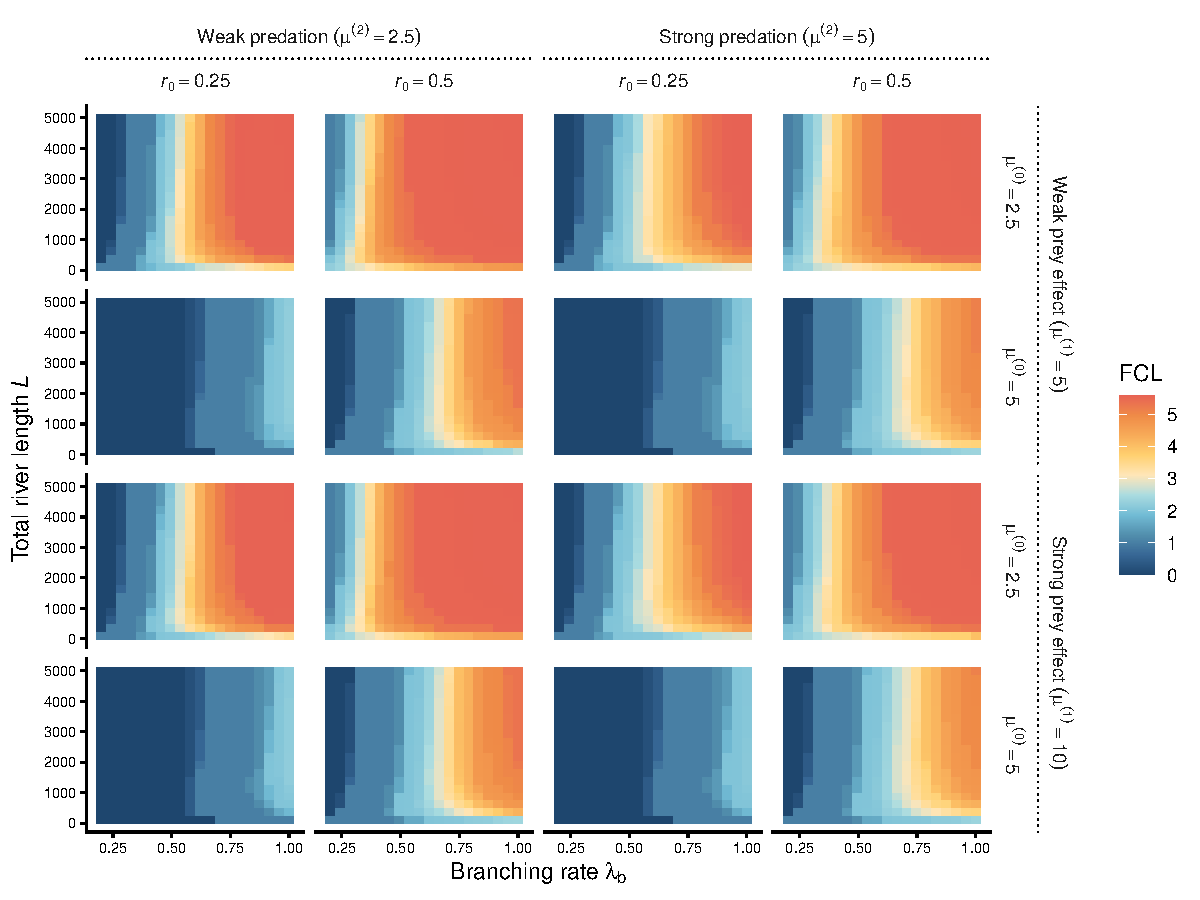
\includegraphics[width=1\linewidth]{tex/fig_theo_delta01_nu01_theta05.pdf}
\caption{Numerical predictions with dispersal decay rate $\delta_0 = 0.1$ (for producers), disturbance decay rate $\nu = 0.1$, and strong omnivory $\theta = 0.5$.Heatmaps of FCL are expressed as a function of ecosystem size (river length, $L$)
and complexity (branching rate, $\lambda_b$), with rows and columns displaying
different combinations of resource supply ($r_0$), disturbance regime
($\mu^{(0)}$), prey effect ($\mu^{(1)}$), and predation effect ($\mu^{(2)}$).
Each cell represents the average FCL of five food webs.
Other parameter values are: producer propagule $g_0 = 5$, habitat density $h = 1$, scaling exponent $\psi = 0.5$.}
\label{fig:fig-num2}
\end{figure}
\newpage

\begin{figure}
\centering
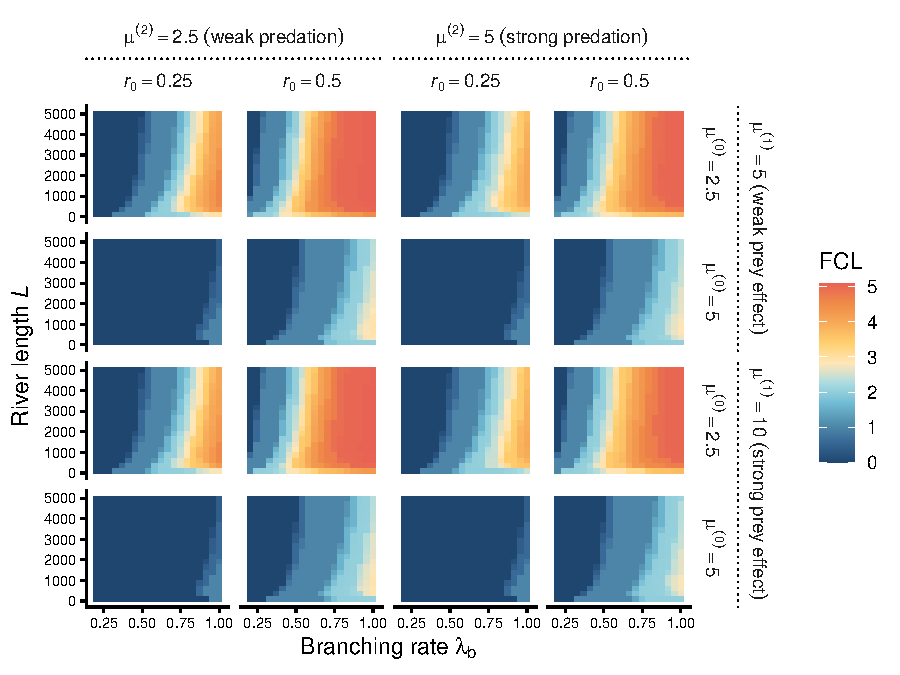
\includegraphics[width=1\linewidth]{tex/fig_theo_delta01_nu005_theta025.pdf}
\caption{Numerical predictions with dispersal decay rate $\delta_0 = 0.1$ (for producers), disturbance decay rate $\nu = 0.05$, and weak omnivory $\theta = 0.25$. Heatmaps of FCL are expressed as a function of ecosystem size (river length, $L$)
and complexity (branching rate, $\lambda_b$), with rows and columns displaying
different combinations of resource supply ($r_0$), disturbance regime
($\mu^{(0)}$), prey effect ($\mu^{(1)}$), and predation effect ($\mu^{(2)}$).
Each cell represents the average FCL of five food webs.
Other parameter values are: producer propagule $g_0 = 5$, habitat density $h = 1$, scaling exponent $\psi = 0.5$.}
\label{fig:fig-num3}
\end{figure}
\newpage

\begin{figure}
\centering
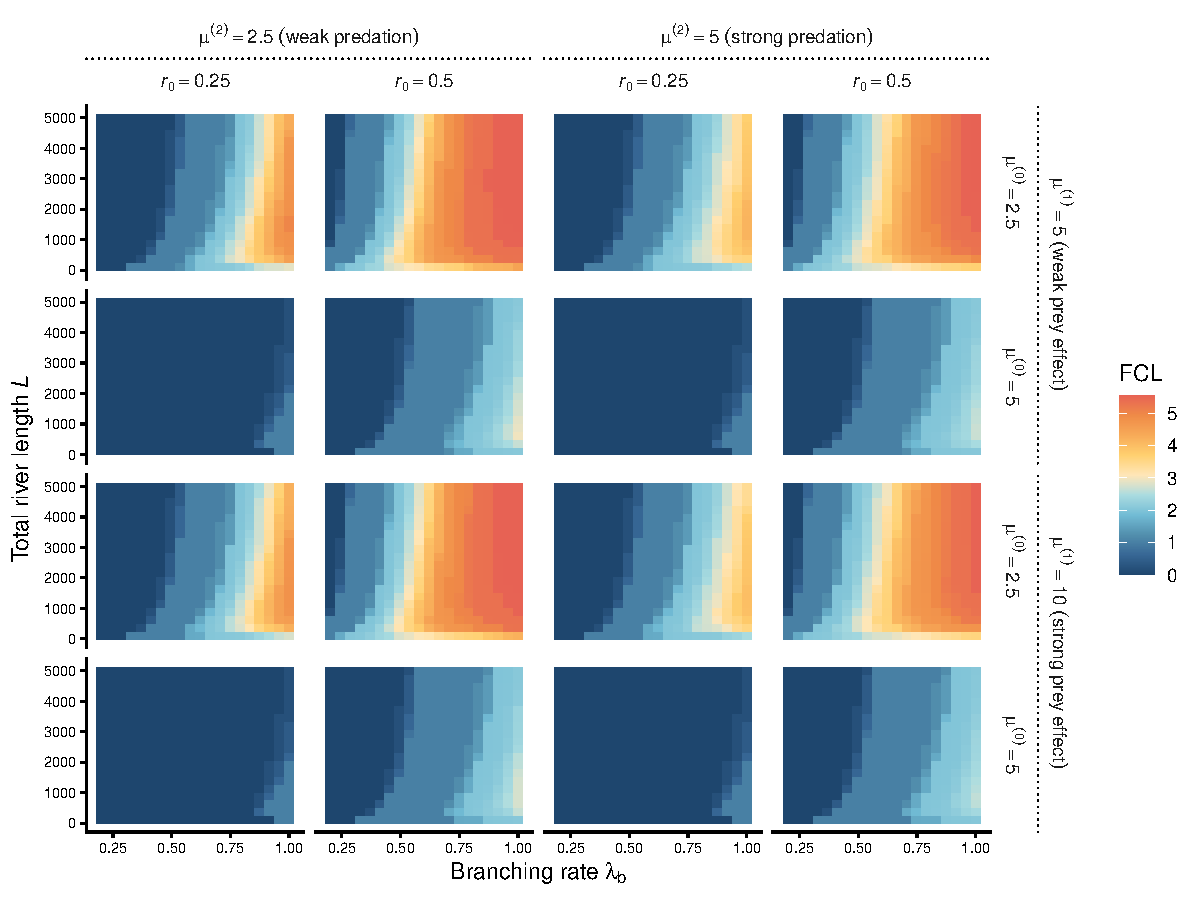
\includegraphics[width=1\linewidth]{tex/fig_theo_delta01_nu005_theta05.pdf}
\caption{Numerical predictions with dispersal decay rate $\delta_0 = 0.1$ (for producers), disturbance decay rate $\nu = 0.05$, and strong omnivory $\theta = 0.5$.Heatmaps of FCL are expressed as a function of ecosystem size (river length, $L$)
and complexity (branching rate, $\lambda_b$), with rows and columns displaying
different combinations of resource supply ($r_0$), disturbance regime
($\mu^{(0)}$), prey effect ($\mu^{(1)}$), and predation effect ($\mu^{(2)}$).
Each cell represents the average FCL of five food webs.
Other parameter values are: producer propagule $g_0 = 5$, habitat density $h = 1$, scaling exponent $\psi = 0.5$.}
\label{fig:fig-num4}
\end{figure}
\newpage

\begin{figure}
\centering
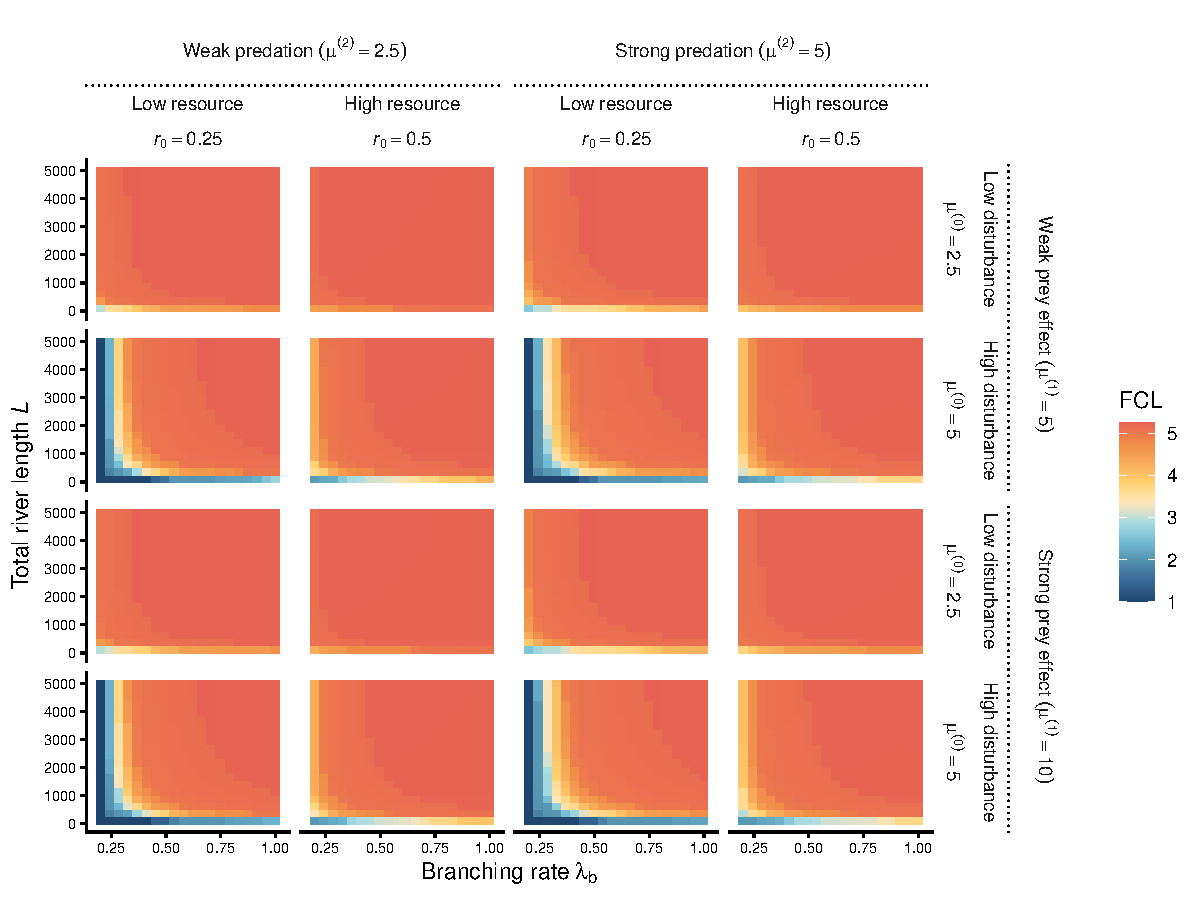
\includegraphics[width=1\linewidth]{tex/fig_theo_delta005_nu01_theta025.pdf}
\caption{Numerical predictions with dispersal decay rate $\delta_0 = 0.05$ (for producers), disturbance decay rate $\nu = 0.1$, and weak omnivory $\theta = 0.25$. Heatmaps of FCL are expressed as a function of ecosystem size (river length, $L$)
and complexity (branching rate, $\lambda_b$), with rows and columns displaying
different combinations of resource supply ($r_0$), disturbance regime
($\mu^{(0)}$), prey effect ($\mu^{(1)}$), and predation effect ($\mu^{(2)}$).
Each cell represents the average FCL of five food webs.
Other parameter values are: producer propagule $g_0 = 5$, habitat density $h = 1$, scaling exponent $\psi = 0.5$.}
\label{fig:fig-num5}
\end{figure}
\newpage

\begin{figure}
\centering
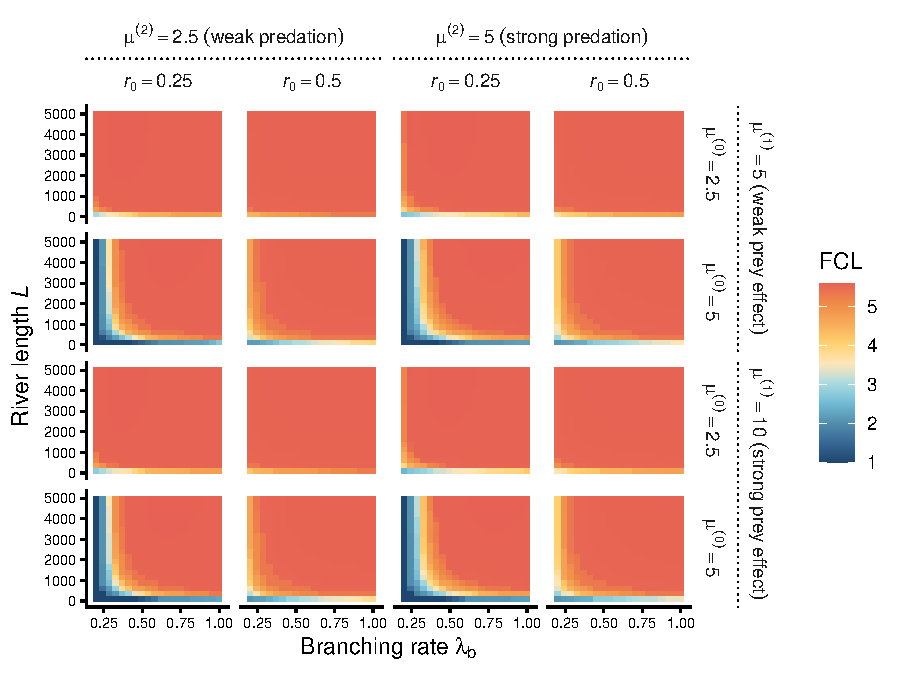
\includegraphics[width=1\linewidth]{tex/fig_theo_delta005_nu01_theta05.pdf}
\caption{Numerical predictions with dispersal decay rate $\delta_0 = 0.05$ (for producers), disturbance decay rate $\nu = 0.1$, and strong omnivory $\theta = 0.5$.Heatmaps of FCL are expressed as a function of ecosystem size (river length, $L$)
and complexity (branching rate, $\lambda_b$), with rows and columns displaying
different combinations of resource supply ($r_0$), disturbance regime
($\mu^{(0)}$), prey effect ($\mu^{(1)}$), and predation effect ($\mu^{(2)}$).
Each cell represents the average FCL of five food webs.
Other parameter values are: producer propagule $g_0 = 5$, habitat density $h = 1$, scaling exponent $\psi = 0.5$.}
\label{fig:fig-num6}
\end{figure}
\newpage

\begin{figure}
\centering
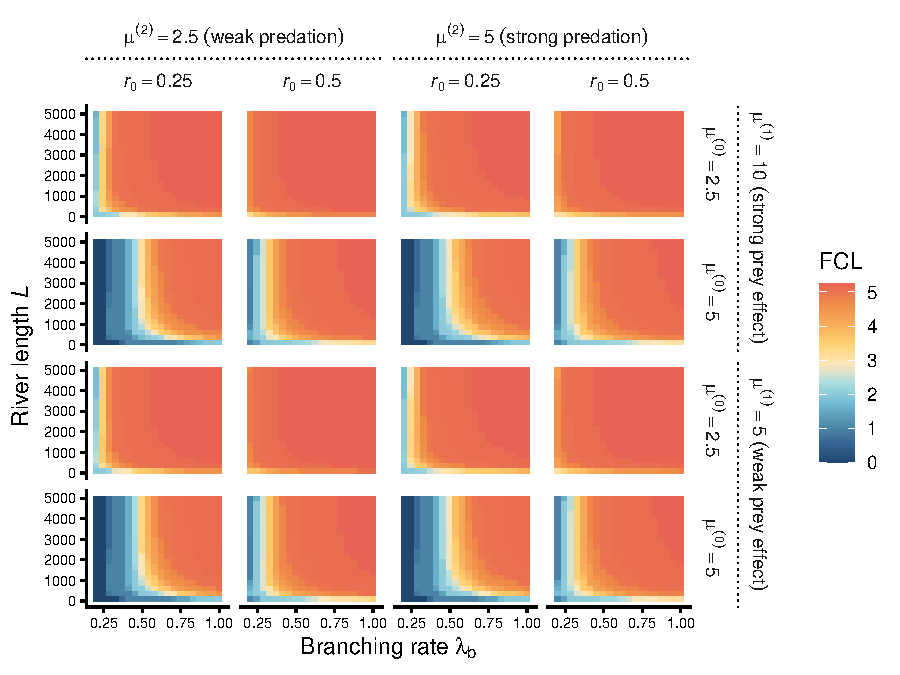
\includegraphics[width=1\linewidth]{tex/fig_theo_delta005_nu005_theta025.pdf}
\caption{Numerical predictions with dispersal decay rate $\delta_0 = 0.05$ (for producers), disturbance decay rate $\nu = 0.05$, and weak omnivory $\theta = 0.25$. Heatmaps of FCL are expressed as a function of ecosystem size (river length, $L$)
and complexity (branching rate, $\lambda_b$), with rows and columns displaying
different combinations of resource supply ($r_0$), disturbance regime
($\mu^{(0)}$), prey effect ($\mu^{(1)}$), and predation effect ($\mu^{(2)}$).
Each cell represents the average FCL of five food webs.
Other parameter values are: producer propagule $g_0 = 5$, habitat density $h = 1$, scaling exponent $\psi = 0.5$.}
\label{fig:fig-num7}
\end{figure}
\newpage

\begin{figure}
\centering
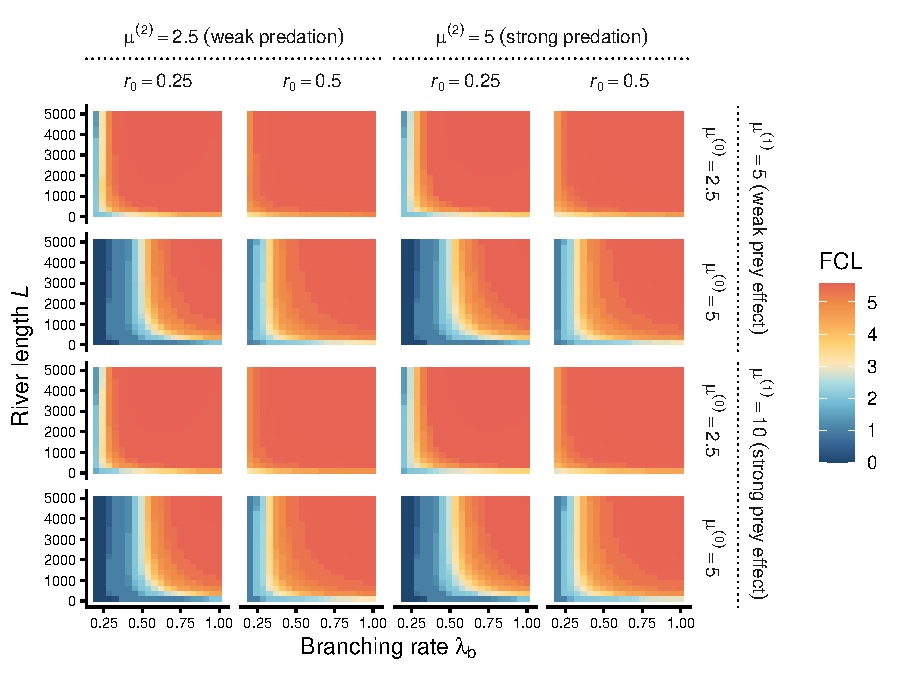
\includegraphics[width=1\linewidth]{tex/fig_theo_delta005_nu005_theta05.pdf}
\caption{Numerical predictions with dispersal decay rate $\delta_0 = 0.05$ (for producers), disturbance decay rate $\nu = 0.05$, and strong omnivory $\theta = 0.5$.Heatmaps of FCL are expressed as a function of ecosystem size (river length, $L$)
and complexity (branching rate, $\lambda_b$), with rows and columns displaying
different combinations of resource supply ($r_0$), disturbance regime
($\mu^{(0)}$), prey effect ($\mu^{(1)}$), and predation effect ($\mu^{(2)}$).
Each cell represents the average FCL of five food webs.
Other parameter values are: producer propagule $g_0 = 5$, habitat density $h = 1$, scaling exponent $\psi = 0.5$.}
\label{fig:fig-num8}
\end{figure}
\newpage

